\documentclass{aidealabs-paper-zh}
% !TeX program = xelatex

\usepackage{xcolor}
\usepackage{pifont}
\usepackage{twemojis}

\title{中文经济学类期刊 \LaTeX 模版}
\author{
    谭淞\thanks{
        谭淞，上海比翼视界信息科技有限公司、上海大学法学院。
        通讯地址：上海市宝山区南陈路333号，Email：sepine@aidea-labs.com。
        该项目为独立的，以 AGPL 3.0 License 为协议的开源项目，旨在让更多人免受排版之苦，普惠研究者。
        项目地址：https://github.com/aidea-labs/econ-sbm-template，
        如模版存在问题或有新的需求，可在该项目中提交 Issue，如您希望贡献代码可根据项目指引提交 PR，
        每一个人的贡献都会使科研更加普惠。}
}
\date{\today}
\addbibresource{ref.bib}

% 下面是特定期刊有要求，可以没有
% \titleen{Templates for Chinese Economics Journals}
% \abstracten{} % 在此填写英文摘要。
% \keywordsen{} % 在此填写三个英文关键词。
% \jel{} % 在此填写三个 JEL 分类号。

\begin{document}

\maketitle

\begin{abstract}
    部分中文经济学期刊尚未提供 \LaTeX{} 模板，研究者在论文写作和投稿时需要自行查找期刊要求并调整稿件格式。
    为减少重复排版工作，本项目整理了若干期刊公开的投稿体例，构建并开源了一系列 \LaTeX{} 模板，尽可能将论文内容与期刊样式分离，方便研究者在同一份稿件上切换模板。
    本文介绍了模板的基本使用方法，以及借助 Git、GitHub 和 AI Agent 进行论文写作、版本管理与协作的方式。
    本项目希望降低社会科学研究者使用 \LaTeX{} 撰写论文的技术门槛，并为不同阶段的写作和投稿提供支持。

\end{abstract}

\keywords{\LaTeX, 学术期刊, 论文排版}

\section{引言}
\label{sec:intro}
\textcite{james_does_2026} 认为使用 \LaTeX 可能提高经济学家对论文研究质量的主观评价。
古语有云：“工欲善其事，必先利其器。\footnote{出自《论语·卫灵公》，其原文为：子贡问为仁。子曰：“工欲善其事，必先利其器。居是邦也，事其大夫之贤者，友其士之仁者。”意思是：工匠要把活干好，必须先让工具锋利；而一个人要在邦国中行仁、干一番事业，就应当去侍奉大夫中的贤能者、结交士人中的仁德之士。}”
一个好的科研工具可以帮助研究者解决中不必要的麻烦，这无疑会提高科研的效率和质量。

\LaTeX 这种为科研排版而生的工具相比于 Microsoft Word （下简称为“MS Word” 或 “Word”）在排版中更胜一筹，且我们不难发现它在给定模版文件的情况下可以轻松地将排版切换至其他期刊。
同时，\LaTeX 这种“源代码-编译-PDF产物”的模式相比于 MS Word 更适合协作和版本追踪。\footnote{更多协作与版本追踪的内容详见第~\ref{sec:github}~节和第~\ref{sec:col}~节。}
此外，它在保持规范化的条件下有更高的灵活性和自由度，表~\ref{tab:word-latex} 对 \LaTeX 和 Word 进行了对比。

\begin{table}[htbp]
    \centering
    \caption{\LaTeX{} 与 Word 在论文写作中的对比}
    \label{tab:word-latex}
    \zihao{5}
    \setlength{\tabcolsep}{3pt}
    \begin{tabular}{@{}p{0.20\linewidth}p{0.38\linewidth}p{0.38\linewidth}@{}}
        \toprule
        \textbf{维度} & \textbf{Microsoft Word} & \textbf{\LaTeX} \\
        \midrule
        \textbf{排版哲学}
          & \textbf{WYSIWYG}（所见即所得），你看到的就是最终打印出来的效果。
          & \textbf{WYSIWYM}（所见即所得意），你只写内容和逻辑结构，由引擎自动排版。 \\
        \addlinespace[2pt]
        \textbf{学习曲线}
          & \textbf{平缓}，上手极快，打开即写，对普通用户极其友好。
          & \textbf{陡峭}，需要学习标记语言、宏包和编译规则，有一定的门槛。 \\
        \addlinespace[2pt]
        \textbf{学习曲线（AI）}
          & AI 较难直接编辑 Word 文档并保留原有格式。
          & AI 可以直接生成和修改源码，作者几乎不需要学习 \LaTeX{} 语法就能开始写作。 \\
        \addlinespace[2pt]
        \textbf{公式与排版}
          & 输入复杂数学公式和大量图表交叉引用时，容易格式错乱或变卡。
          & \textbf{专业且完美}，极其擅长排版长篇巨著、复杂公式、多级定理与交叉引用。 \\
        \addlinespace[2pt]
        \textbf{协作与审阅}
          & \textbf{强}，支持多人实时在线协作、批注、修订（Word/Office 365）。
          & \textbf{代码式协作}，基于纯文本（如 Overleaf 或 Git 版本控制），类似写代码的分支与合并。 \\
        \addlinespace[2pt]
        \textbf{文件格式}
          & 复杂混合格式。
          & \textbf{纯文本文件}（\texttt{.tex}），轻量。 \\
        \addlinespace[2pt]
        \textbf{版本管理}
          & 不方便做细致的版本 Diff。
          & 天然契合 Git 等版本管理工具。 \\
        \addlinespace[2pt]
        \textbf{适用场景}
          & 日常办公、商业报告、简单论文、简历、图文混排、快速修改。
          & 学术论文、学位论文、书籍，以及含有大量公式或交叉引用的科技文档。 \\
        \bottomrule
    \end{tabular}
    \par\smallskip
    {\footnotesize\raggedright
    \textbf{注：}该对比内容由 Gemini 生成，可以代表作者部分观点\par}
\end{table}


在 AI 的辅助中，文档的存储结构影响模型获取和修改文本的方式。
Word 的 \texttt{.docx} 文件采用 Office Open XML（OOXML）格式，正文和样式信息以 XML 形式存储。
提取正文时，需要将分布在多个 XML 节点中的文本片段按文档顺序拼接。
而 \LaTeX 源文件采用纯文本格式，正文内容与排版命令可在同一文件或不同文件中读取，使得内容与格式配置可以解耦，整体版式也可由文档类统一管理。
这种结构有助于简化文本提取流程，使研究者或者模型能够直接在源文件中定位和修改内容。
此前，我们针对于 AI 的能力写过一篇如何让社科研究者用好 \LaTeX 的研究博文，
感兴趣者可以\href{https://marx-max.aidea-labs.com/blog/2026-10-26-latex-guide-social-scientists/}{点击这里查看}。

尽管 \LaTeX 的优势有这么多，但依旧遗憾的是我们在调查了大量的经济学中文期刊后发现，极少数的期刊提供了 \LaTeX 模版，为了让更多的研究者能够从 \LaTeX 中受益，我们做了该项目并决定开源出来。
该项目所采用的开源协议为 \href{https://github.com/aidea-labs/econ-sbm-template?tab=AGPL-3.0-1-ov-file}{AGPL 3.0 License}\footnote{GNU AFFERO GENERAL PUBLIC LICENSE Version 3（AGPL v3.0 License）允许使用、复制、修改和再分发受其约束的作品。分发修改版时，应按同一许可证授权，并依其条款提供相应源代码。若修改版支持通过网络与用户交互，还须向这些用户提供获取相应源代码的途径。}，该许可证允许任何研究者使用该模版。

该项目的边际贡献主要体现在如下三个方面：
（1）针对部分没有提供 \LaTeX{} 模板的中文经济学期刊，本项目参考其公开的投稿要求制作了相应模板，减少研究者自行调整格式的工作；
（2）本项目参考并整合已有模板，尽可能将论文内容与期刊样式分离，使研究者可以在保留同一份论文内容的基础上切换模板；
（3）本项目同时为社会科学研究者提供了一套需要较少技术的 \LaTeX{} 食用方式，介绍公式、图表和文献引用，以及借助 GitHub 和 AI Agent 进行写作与协作的方法（搭配麦当劳薯条 \twemoji{french fries} 食用更美味，此处无广告）。

本文剩余部分安排如下。
第~\ref{sec:works}~章介绍与本项目潜在相关的工作，包括 AEA 的审阅模式和一些 AI Agent 的基础知识。
第~\ref{sec:use}~章介绍如何使用本项目：首先在第~\ref{sec:github}~节介绍 Git 和 GitHub，随后在第~\ref{sec:how}~节介绍如何使用模板撰写论文，最后在第~\ref{sec:col}~节介绍如何通过 GitHub 与合作者共同完成论文。
第~\ref{sec:conclusion}~章对全文进行总结，并讨论项目的局限与后续工作。

\section{相关工作}
\label{sec:works}

\subsection{双倍行距的审阅模式}
% 先讲一下为什么 edit 模式是双倍行间距，这个就不得不讲我用 AEA 的模版写 paper 的时候了，套上模版感觉哪里不对劲，然后发现它有一个审阅的模式，这东西是真好，真的好，真的真的真的好。
本项目建议在写作时采用审阅模式（\texttt{edit}），这一设计源于我在使用美国经济学会（American Economic Association，AEA）的 \LaTeX{} 模板写作时的体验。
AEA 为投稿作者提供了审阅模式，并要求使用其模板准备投稿稿件时采用该模式。\footnote{AEA 模板说明见 \url{https://www.aeaweb.org/journals/templates}。}
初次套用模板时，我注意到稿件的行距明显变大，后来才发现这是审阅模式的排版设置。
较宽的行距让阅读和批注有了更多空间，也方便作者逐段检查和修改。
因此，本项目在审阅模式中采用双倍行距，作为研究者撰写、讨论和修改稿件时的默认版式。

对我个人而言，我喜欢将论文打印出来，用纸笔阅读和修改。
纸质稿上的批注可以直接写在需要调整的句子旁边，遇到需要重新组织的论证，也可以在段落间标记调整思路。
双倍行距为这些修改留出了书写空间，使添加词句、修改措辞和标记问题时不必将文字挤在一起。
对于需要多轮修改的稿件，这样的排版也方便作者回看此前留下的批注。

在对研究者的调研中，我发现，喜欢打印稿件阅读和修改的并不只有我一人。
他们同样需要在纸质稿上留出批注和修改的空间。
这意味着，审阅版式需要考虑纸笔修改的空间。
双倍行距的审阅模式为这些研究者提供了一份适合打印批注的稿件，也让纸质审阅中留下的意见更容易在后续修订时辨认和整理。

现有文献也能支持打印的纸质版是文献阅读的一种主要方式。
\textcite{tenopir_international_2019} 在 2018 年开展了一项国际调查，要求受访者回忆最近一次阅读学术文章的方式。
在回答该问题的 366 名受访者中，有 133 人将下载的文章打印后阅读，占比约 36.3\%。
调查共获得 606 份有效回应，其中约三分之一的受访者来自社会科学领域，但作者指出该样本可能不具代表性。
在另一项芬兰调查中，\textcite{tenopir_finland_2019} 记录了研究者于 2016 年报告的最近一次期刊文章阅读经历。
在 455 次阅读中，40.4\% 是将下载的文章打印后阅读，另有 5.3\% 直接阅读纸质期刊。
这些结果表明，纸质阅读在两项调查记录的学术阅读中占有一定比例，为关注研究者的纸质阅读需求提供了经验依据。

纸质批注也出现在已有调查中。
\textcite{lincoln_reading_2013} 对神学和宗教研究领域的图书馆用户进行调查，发现教授或讲师受访者中有 53\% 表示经常在纸质文章上批注或标记重点。
在德国职业教育与培训研究领域的调查中，\textcite{getz_researchers_2021} 报告有 63.6\% 的受访者同意或倾向同意，自己阅读纸质材料时比阅读屏幕上的数字出版物更专注。
对于习惯纸质阅读和批注的研究者，审阅模式可以直接生成双倍行距稿件，使得打印后的阅读效果更舒服。

\subsection{Agent Skill}

Agent Skill 是由 Anthropic 于 2025 年推出的一种面向 AI Agent 提供特定任务知识与操作流程的开放格式。
一个 Skill 通常以文件夹的形式组织，其中的 \texttt{SKILL.md} 文件描述该技能的名称、用途和执行说明，也可以附带脚本、参考资料或模板等资源。\footnote{更多信息详见 \url{https://agentskills.io} 和 \url{https://github.com/anthropics/skills}。}
当用户的任务与某项技能相关时，Agent 可以读取相应说明和所需资源，并据此完成任务。
这种组织方式使研究者能够将常用的操作步骤和领域知识保存下来，在后续任务中重复使用。


在实际写作中，\LaTeX{} 的编译命令和环境配置并不容易记住，遇到又臭又长的报错日志时，找到问题所在也可能需要花费不少时间。
有一天我发现，ChatGPT Desktop 中有一个 OpenAI 发布的 LaTeX 插件，可以协助处理这些工作（见图~\ref{fig:latex-plugin-openai}）。\footnote{如果你的 ChatGPT 里还没有这个插件，可以尝试发送这样的提示词：“请从 \url{https://chatgpt.com/plugins/share/latex@openai-bundled} 安装 LaTeX 插件，并帮我检查我的 LaTeX 环境是否准备就绪。”}
这个插件包含三个 Skill：\texttt{latex-doctor} 用于检查编译环境和工具是否可用，\texttt{latex-compile} 用于编译稿件，\texttt{texlive-runtime-installer} 则在没有检测到可用的 TeX Live 或 MacTeX 时，帮助安装完整的 TeX Live 环境。
借助这些技能，研究者可以用自然语言请 Agent 检查环境、编译文件并协助分析报错，把更多精力放在论文内容上。

\begin{figure}[htbp]
    \centering
    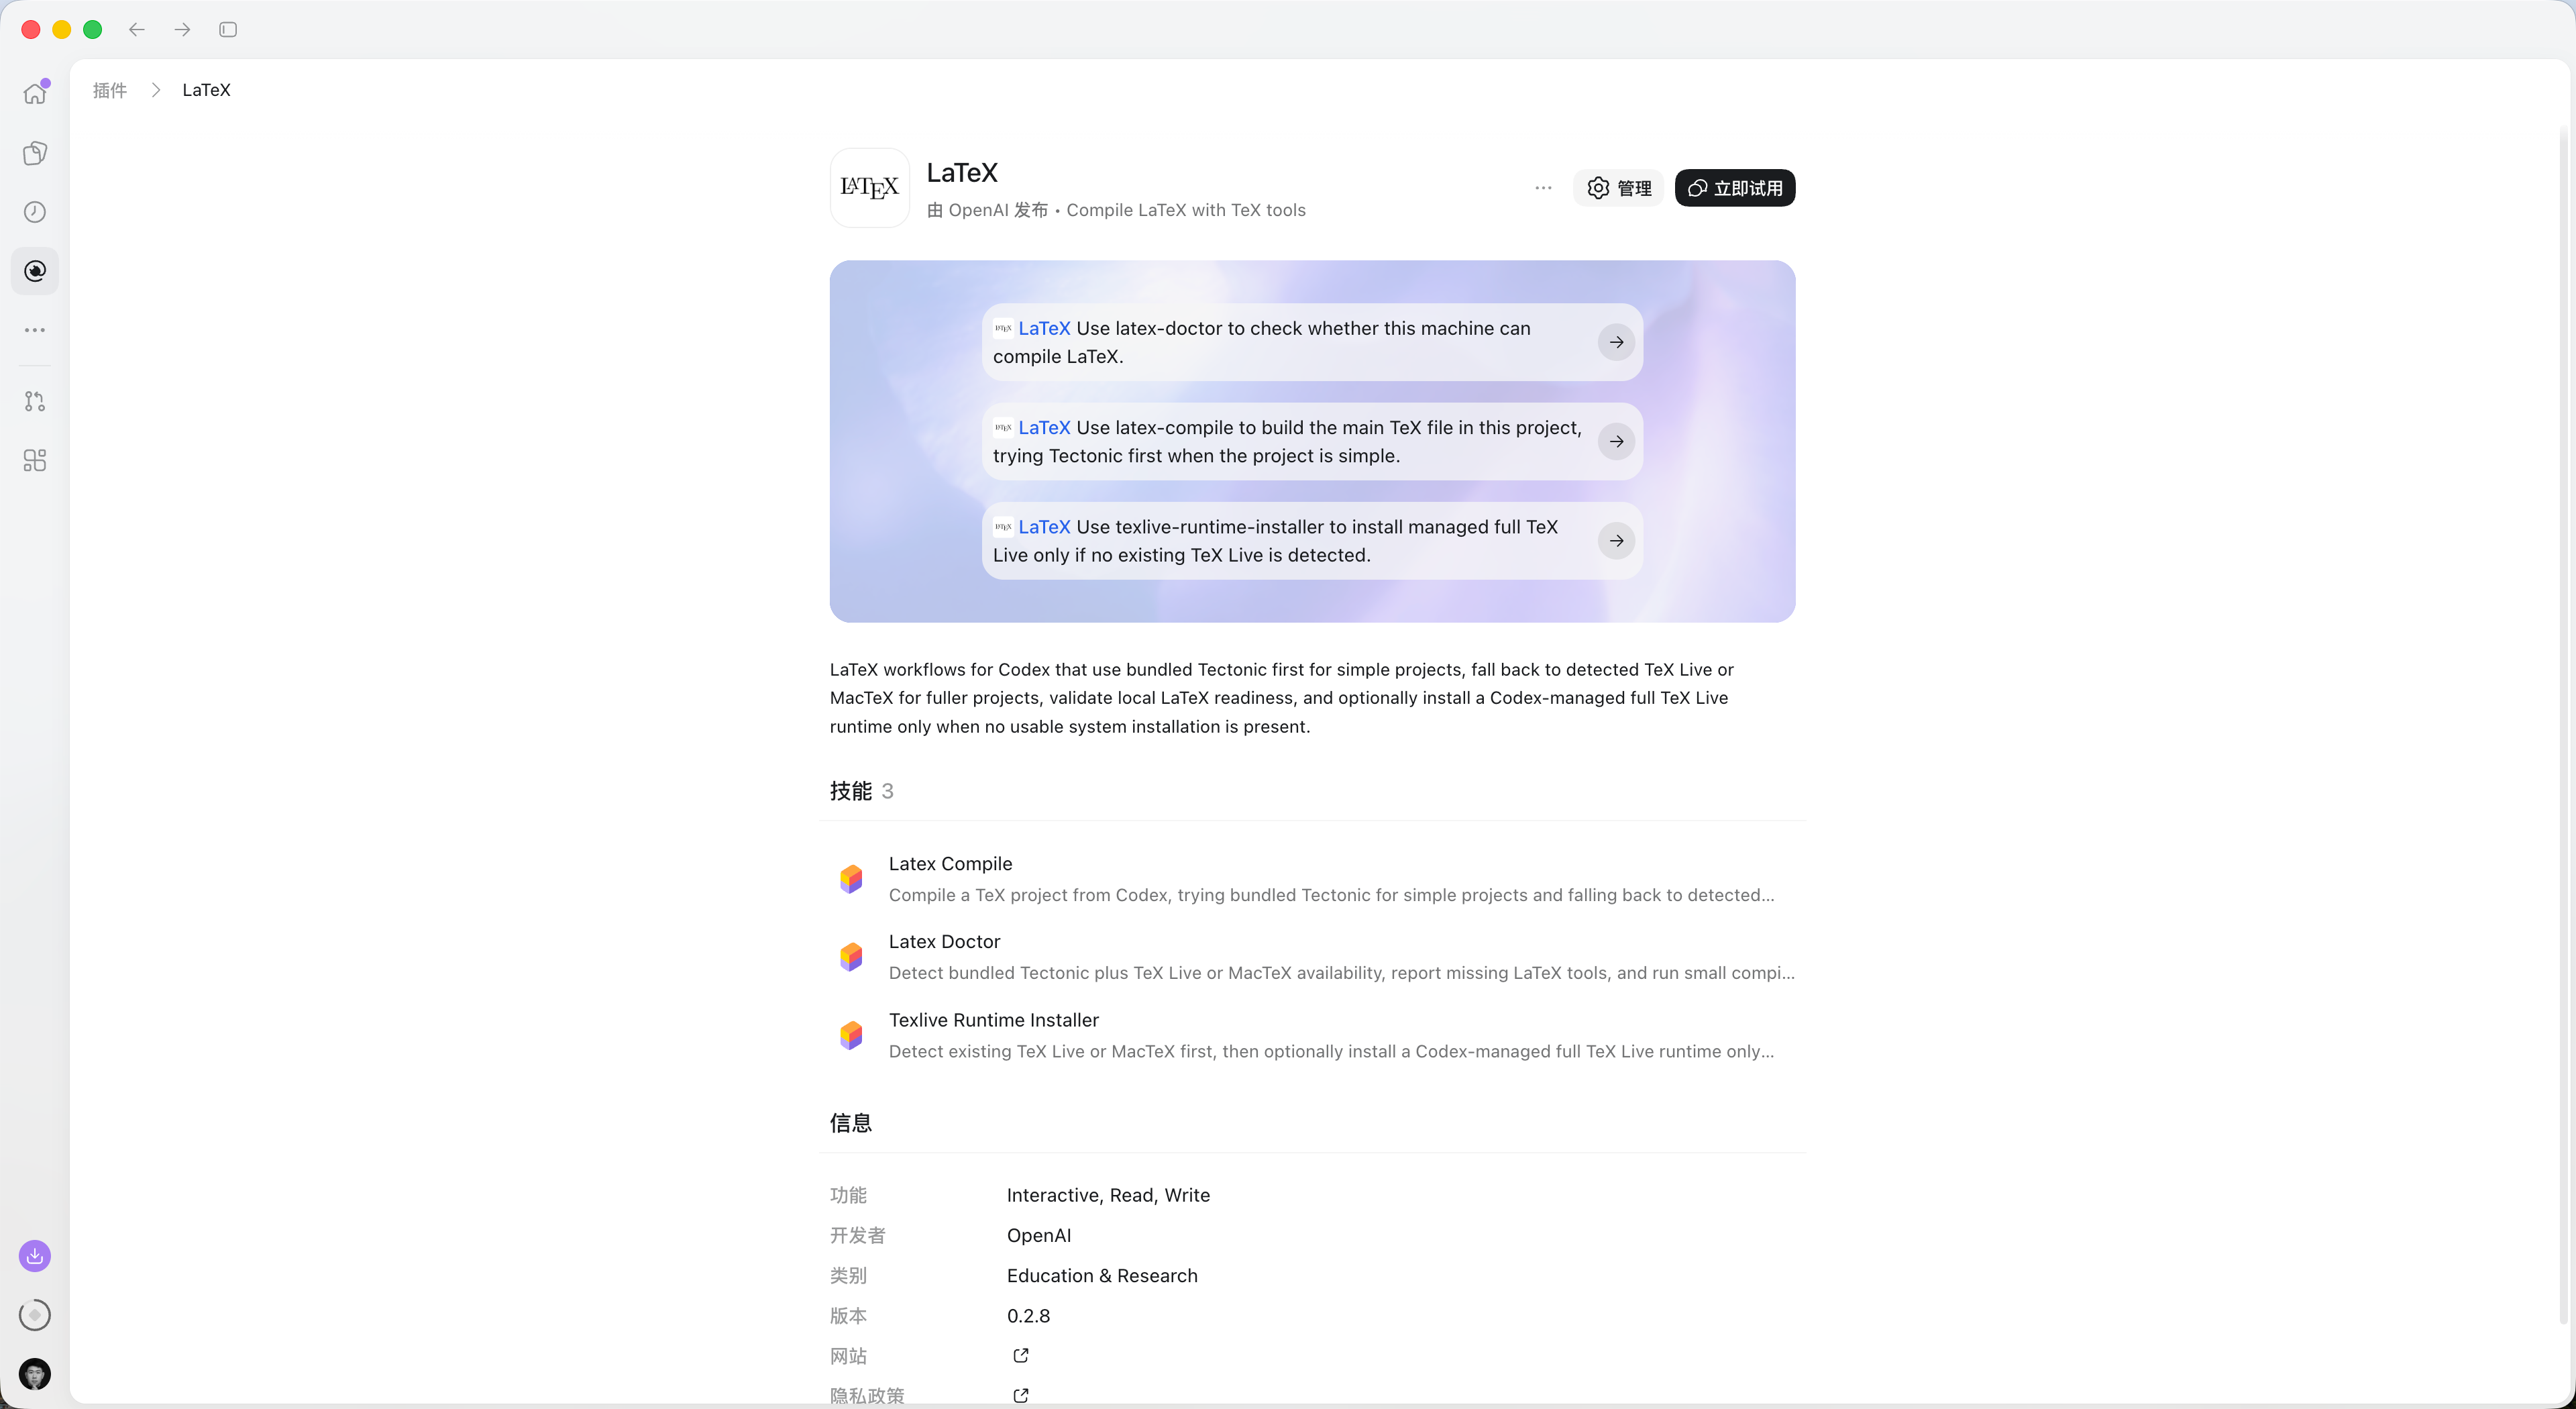
\includegraphics[width=\linewidth]{figs/latex-plugin-openai.png}
    \caption{OpenAI 发布的 \LaTeX{} 插件及其附带的三个 Skill}
    \label{fig:latex-plugin-openai}
\end{figure}


同时，因为我并没有找到特别好用特别适合我的 Skill 来帮我处理具体的命令。
因为我记不住 \LaTeX{} 的命令，所以我需要借助于 AI 帮我写很多的命令。但当我处于无网络的情况下我不得不依赖于我在本地部署的模型，可他们的能力却一言难尽。
因此，在我开源的一套 Agent Skill 里有一个专门的 Skill 就是针对于如何编写 \LaTeX{} 代码。
该 Skill 面向论文写作中常见的 \LaTeX{} 代码编写任务，整理了公式、图表和文献引用等场景的基本写法及注意事项。\footnote{项目地址为 \url{https://github.com/sepinetam/sepine-research-skill}。如需安装只需要将下面这段话发给你的 Agent：“帮我安装 Sepine 的 Research Skill，地址在 https://github.com/sepinetam/sepine-research-skill”}
使用时，我们只需要用自然语言讲出我们需要什么样的效果，Agent 即可结合 Skill 中的说明生成或修改相应代码。
对于本地部署的模型，这些说明也可以作为完成任务时的参考，帮助它按照项目约定处理常见的 \LaTeX{} 命令。

\subsection{Coding Agent}

Coding Agent 是一种能够围绕用户提出的任务，结合项目文件编写、修改和运行代码的 AI Agent。
研究者可以用自然语言描述问题，让它读取相关文件、生成程序、执行命令，并根据运行结果继续调整。
在论文写作场景中，这种工作方式也可以用于编辑 \LaTeX{} 源码、编译稿件和排查编译错误。

\textcite{lyttelton_coding_agents_2026} 对 1,260 名定量社会科学研究者开展的基线调查发现，81\% 的受访者曾在研究中使用生成式 AI，而约 20\% 经常使用 Coding Agent。
研究同时指出，受访者是为一项提供 Claude 使用机会的研究招募的，并不构成具有代表性的总体样本。
另一项研究中，\textcite{hermle_scientific_discovery_2026} 分析了 207,000 个 Claude 和 Claude Code 科研会话，发现数据分析约占 Claude Code 科研会话的一半。
这些结果反映了研究者使用相关工具的场景，为理解 Coding Agent 在科研工作中的应用提供了线索。

在研究的具体环节中，AI Agent 可以围绕数据、代码和运行结果协助研究者完成任务。
例如，在数据整理阶段，\textcite{li_autodcworkflow_2025} 构建了 AutoDCWorkflow，根据原始表格和分析目的生成数据清洗步骤，并在涵盖 96 张表格、142 个分析目的的测试集中评估了结果。
在研究复现阶段，\textcite{shah_reproducibility_2026} 以五项原本可以复现的社会科学研究为基础，人为加入缺失软件包、文件路径错误等问题，考察 Agent 检查文件、修改代码并重新运行分析的能力。
在这组受控测试中，Agent 方案在不同难度下的复现成功率为 69\%--96\%，展示了它协助处理分析流程中具体错误的可能性。
从数据整理到程序运行和复现检查，这些工作为研究者如何借助 Agent 处理实证研究中的重复性任务提供了参考。
研究者仍需要结合研究问题判断数据处理规则、样本与模型设定，并检查 Agent 生成的代码和结果。

对于希望在研究中使用 Coding Agent 的研究者，目前已经有几种通用工具可以选择。
目前比较主流的解决方案详见表~\ref{tab:agents}，其中主要推荐的智能体有 ChatGPT Desktop 和 DeepSeek Harness。\footnote{这两个 Agent Harness 的推荐考量是从可用性和可付费性两个角度。我们不得不承认 Claude 很强，但受限于某些许可的原因身处于中国大陆的用户不能够进行购买和使用，但与之相对应的 ChatGPT 就会缓和很多，可以相对轻松地使用上和订阅上。DeepSeek Harness 是完全开源的 Harness 框架，其推荐原因是它的新颖性和被爱包裹，一个在爱中长大的孩子，被整个社区用爱投喂，它差不到哪去。}
ChatGPT Desktop 中有两种模式，分别为 ChatGPT 和 Codex，我们可以简单地用一个通俗的方式去理解，ChatGPT 主要赋能工作场景（或轻代码场景），聚焦于将重复化的工作流自动化；Codex 更多赋能于编码场景。对于研究者来说，如果是资深研究者可以考虑从 ChatGPT 模式切入，在协作工作中把固定的流程自动化。
DeepSeek Harness 我们可以简单地理解成电脑界的 Linux，手机界的 Android，（汽车界的 Tesla？）它有高度化的自定义能力，适合喜欢折腾的研究者。它就好像是给你一间毛坯房，你可以自由地配置任何事物只要你能想到。

\begin{table}[htbp]
    \centering
    \caption{几种 AI Agent 工具的比较}
    \label{tab:agents}
    \zihao{5}
    \setlength{\tabcolsep}{3pt}
    \begin{tabular}{@{}p{0.19\linewidth}p{0.16\linewidth}p{0.39\linewidth}p{0.20\linewidth}@{}}
        \toprule
        \textbf{名称} & \textbf{来源} & \textbf{特点} & \textbf{可获得性} \\
        \midrule
        ChatGPT & OpenAI & Codex 内核开源 & \ding{72}\ding{72}\ding{72}{\color{gray}\ding{72}\ding{72}} \\
        \addlinespace[2pt]
        Claude & Anthropic & Claude Code 编程与命令执行 & \ding{72}{\color{gray}\ding{72}\ding{72}\ding{72}\ding{72}} \\
        \addlinespace[2pt]
        DSH & DeepSeek & 完全开源、一切皆插件 & \ding{72}\ding{72}\ding{72}\ding{72}\ding{72} \\
        \addlinespace[2pt]
        WorkBuddy & 腾讯 & 办公与文件处理 & \ding{72}\ding{72}\ding{72}\ding{72}\ding{72} \\
        \addlinespace[2pt]
        豆包工作 & 字节跳动 & 办公与飞书生态 & \ding{72}\ding{72}\ding{72}\ding{72}\ding{72} \\
        \addlinespace[2pt]
        Marx Max & AIdea-Labs & 专为社科研究者制作 & \ding{72}\ding{72}\ding{72}\ding{72}{\color{gray}\ding{72}} \\
        \bottomrule
    \end{tabular}
    \par\smallskip
    {\footnotesize\raggedright
    \textbf{注：}可获得性满分五颗星，黑色星表示所得星数，灰色星表示其余星数。\par}
\end{table}


除此之外，我们在打造一个专门为社会科学研究者服务的 AI 原生科研工作台。\footnote{目前仍在开发测试阶段，欢迎有兴趣的研究者来尝试使用，产品名字暂定为 Marx Max，名字的灵感源自两位社会科学的巨人，卡尔·马克思和马克思·韦伯。详见\href{https://marx-max.aidea-labs.com/?source_utm=econ-sbm-template}{\underline{\textit{产品官网}}}}
在该产品中，我们将对话、文件系统、科学计算、文献管理等科研常用工具集成在同一个桌面环境，它可以视为社会科学版的 Claude Science，让研究者能够围绕自己的数据、代码和稿件等内容在同一处推进。
该项目的出发点是不希望让“贩卖焦虑”的自媒体对科研产生不当的影响。
我自己平时刷手机的时候，发现很多的账号在渲染一种“再不学习就被淘汰了”的观点，起初我以为不会有人陷入其中，但是事实却让我愕然。
我认为，当下的 AI 对于研究者来说是一种“现在不学就不需要学”的状态，因为技术的变化实在是太快了，我们不可能在研究之外每天都去追最新的技术，而如果晚一两周再去看一项新技术的话，它可能已经被革新了。

故此，我希望能够让技术平权，让每一个研究者可以专注于自己的研究上而非被这种 FOMO 的情绪左右。
我们不希望让它们渲染这种情绪，它们可以不要 reputation，但是我们不能。
不同的研究者有着不同的编程经验、时间和技术资源，配置环境、选择工具和排查错误也需要花费不少精力。
我们希望通过整合科研中常用的工具，让研究者能够从自己熟悉的数据整理、文献阅读和论文写作等任务出发使用 AI Agent，并查看其执行过程和结果。
研究者可以根据自己的需要决定是否使用这些工具，以及如何使用它们，而不必因为缺少技术经验就被挡在门外。
这个大项目是一场马拉松，从社会科学研究的实际过程出发，降低使用 AI Agent 处理科研任务时的操作门槛，让研究者能够将精力更多地放在研究问题和结果判断上。

\section[\LaTeX 极速入门]{\LaTeX 极速入门\protect\footnotemark}
\footnotetext{该部分的内容为科普向，如已对 Git，GitHub，LaTeX 均已熟悉，可略过该章}
\label{sec:use}

\subsection{Git 与 GitHub}
\label{sec:github}

Git 是一种版本控制工具，用于记录文件在不同时间的修改情况。
我们可以用它来保存论文和分析代码的修改历史，比较不同版本之间的差异，并在需要时找回此前的内容。
更直观地讲，它是一个手动触发的时光机。
例如，我们在调整样本范围并重新估计模型后，可以将相关修改提交，后续如果发现问题，可以找回之前版本的代码，而不需要用诸如 \texttt{final-261111-real-final-v10-打死都不改了版-再改就吐血了.docx} 这样的命名存档。

我们也可以用数学语言进行介绍，设第 $t$ 次提交所记录的文件状态为 $S_t$，从该版本到下一版本的改动为 $\Delta_t$。在沿同一条分支持续修改的情况下，下一版本可以表示为
\[
    S_{t+1} = \mathrm{Apply}(S_t, \Delta_t).
\]
其中，$\mathrm{Apply}$ 表示将改动应用到文件上。Git 的每次提交可表示为
\[
    C_t = (S_t, P_t, M_t).
\]
$S_t$ 是提交时的文件快照，记录的是版本控制中已跟踪文件的状态，以及本次提交中新增或修改的文件；尚未加入提交的修改和被忽略的文件不会自动保存。
$P_t$ 是该次提交直接接续的提交集合，$M_t$ 包含作者、时间和修改说明。

若每次提交都接续上一次提交，版本历史形成一条链
\[
    C_0 \longrightarrow C_1 \longrightarrow C_2.
\]
若两位合作者从同一版本 $C_0$ 出发，分别修改正文和分析代码，再将两人的修改合并，并生成一个合并提交，版本历史可以表示为
\[
    C_0 \longrightarrow
    \left\{
    \begin{array}{l}
        C_1^{(A)} \\
        C_1^{(B)}
    \end{array}
    \right\}
    \longrightarrow C_2^{(\mathrm{merge})}.
\]
其中，合并提交 $C_2^{(\mathrm{merge})}$ 同时接续 $C_1^{(A)}$ 和 $C_1^{(B)}$。由此，Git 的版本历史可以表示为有向无环图，其中每个节点对应一次提交，箭头从较早的提交指向接续它的提交。

GitHub 是一个基于 Git 的在线托管与协作平台。
研究者可以将论文的 \LaTeX 源文件、参考文献和分析代码放在同一个仓库中，与合作者共享。
合作者可以在线查看每次提交改动了哪些文件，也可以提交拟议的修改，由其他成员审阅和讨论后再将其纳入共同维护的稿件。

研究者可以使用 GitHub 上的模板仓库创建自己的论文项目。
这里以图~\ref{fig:github-paper-template} 所示的 AIdea-Labs 内部模板为例，点击页面右上方的 \textbf{Use this template}，再选择 \textbf{Create a new repository}，即可在自己的账户下新建一个包含该模板项目文件的新仓库。
新仓库从一条初始提交开始，与原模板仓库不共享提交历史，此后可以独立记录论文的修改过程。
如果你希望向模板仓库贡献修改，可以通过 \textbf{Fork} 按钮创建一个与原仓库关联的副本，在自己的副本中修改后，向原项目提交 \textbf{Pull Request}（简称 PR），请求维护者检查并合并这些修改。
由于基于模板创建的仓库与原仓库没有共同的提交历史，通常不能直接向原模板仓库提交 PR。
因此，使用模板写自己的论文可以选择 \textbf{Use this template}，向模板项目贡献修改则可以选择 \textbf{Fork}。

\begin{figure}[htbp]
    \centering
    \setlength{\unitlength}{\linewidth}
    \begin{picture}(1,0.501)
        \put(0,0){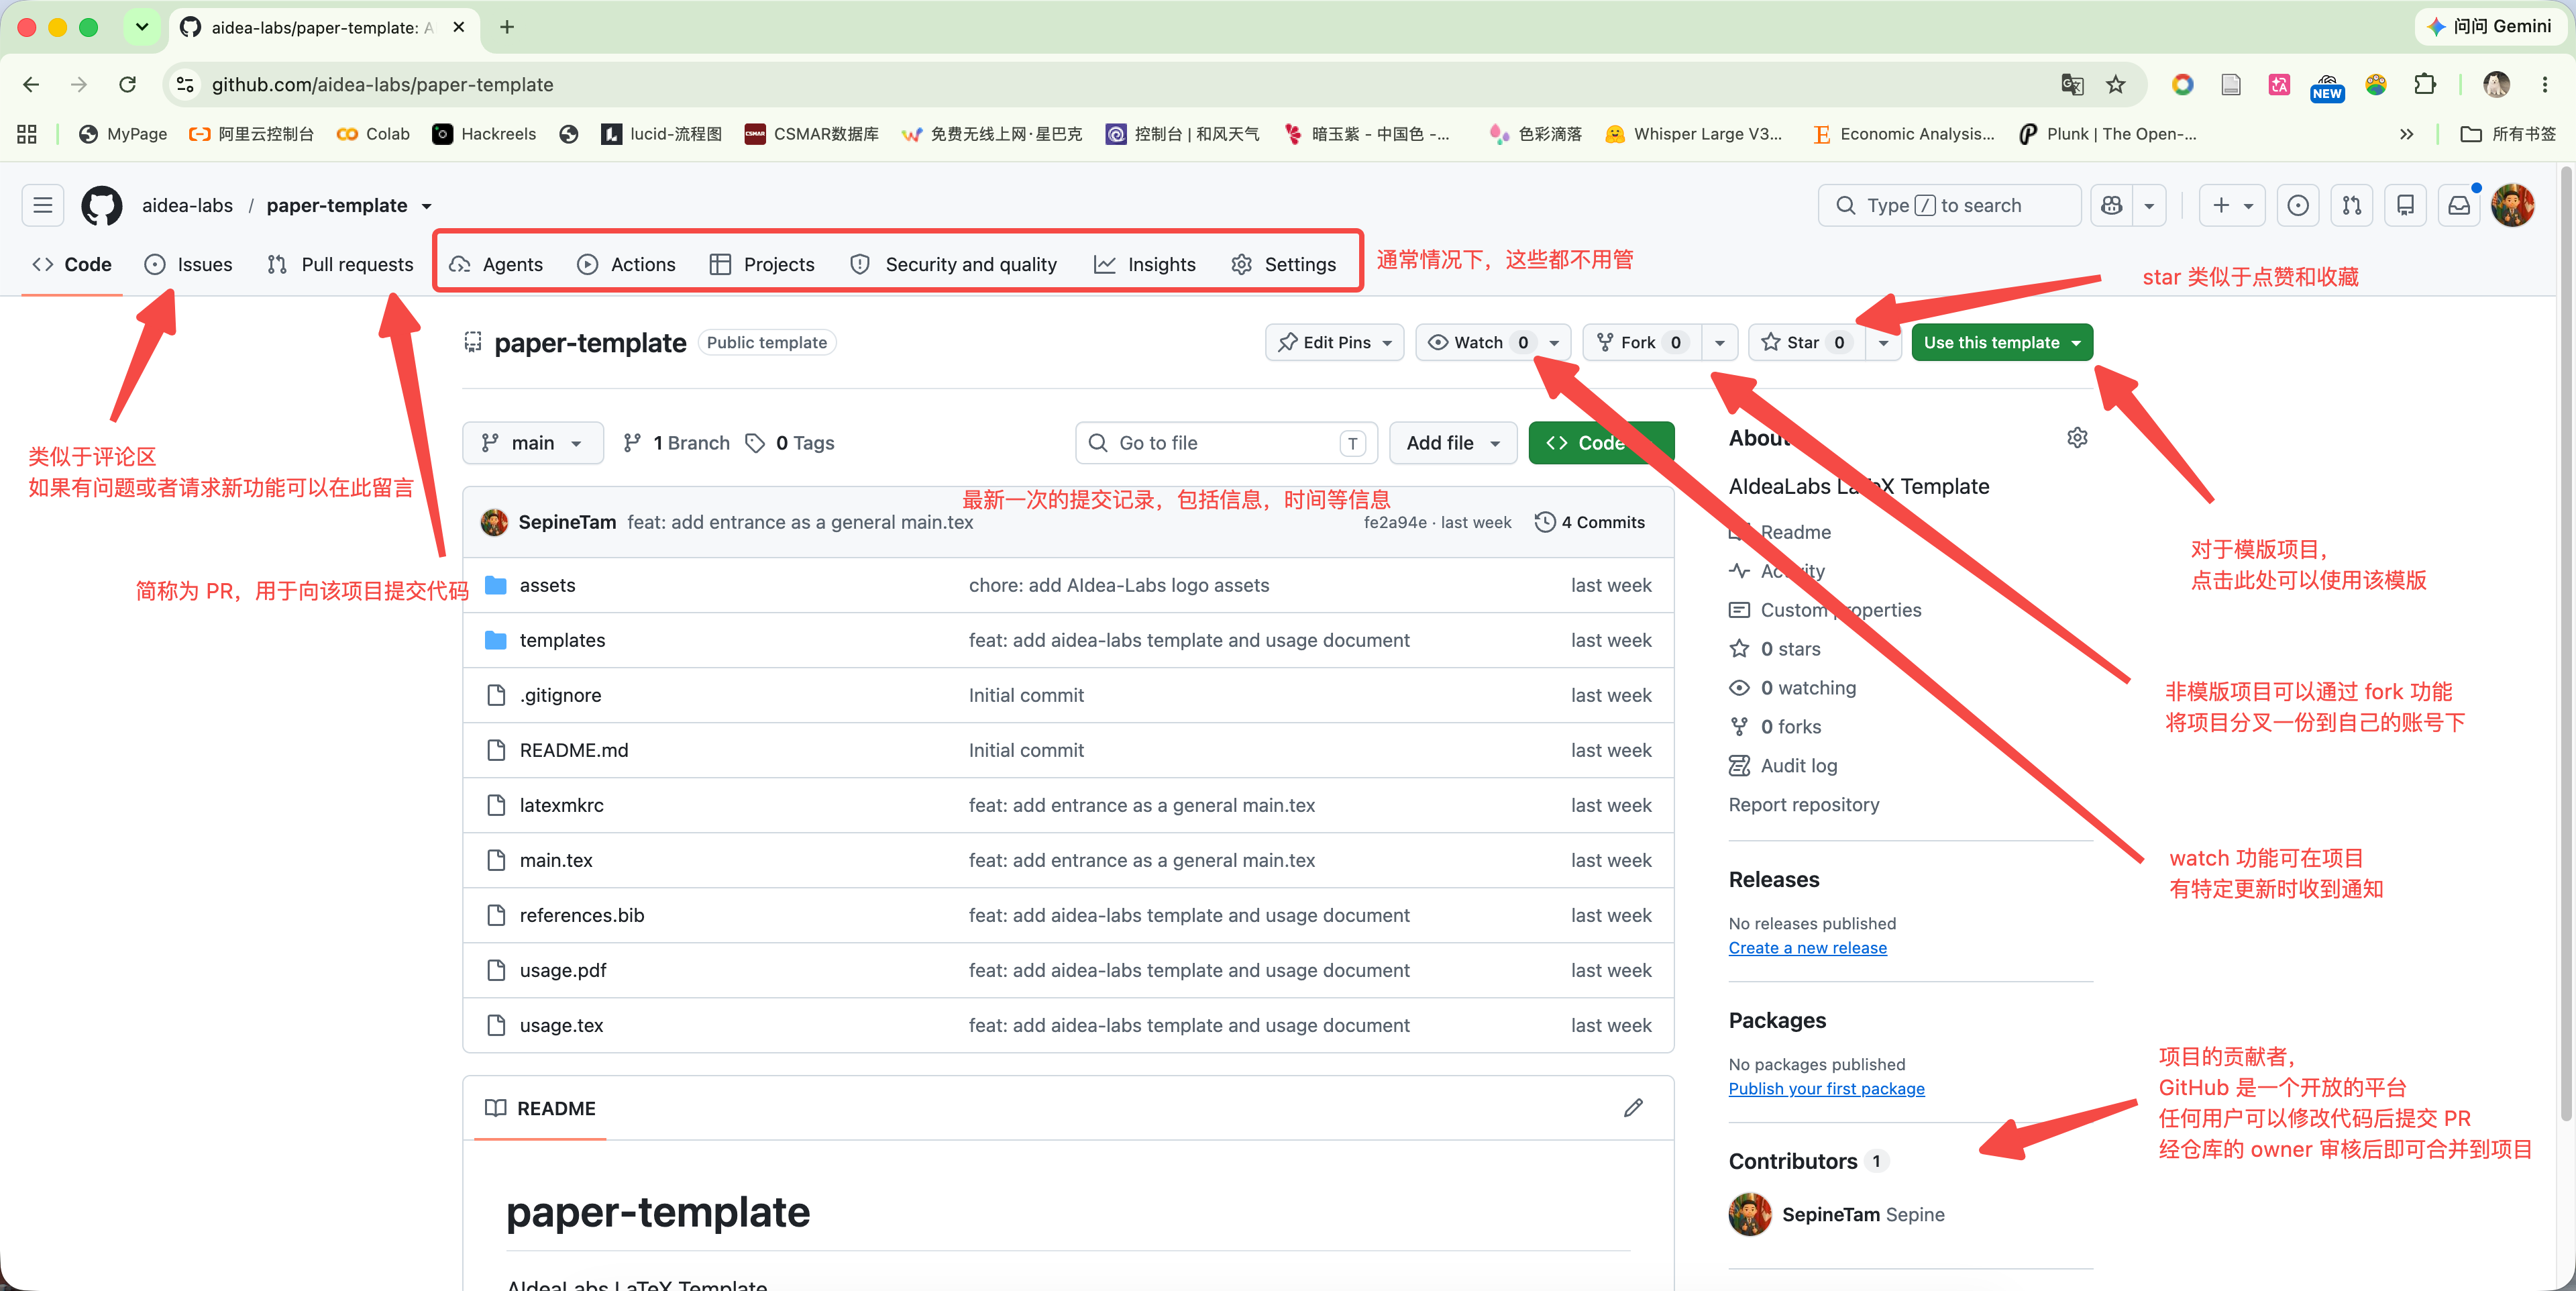
\includegraphics[width=\linewidth]{figs/github-paper-template.png}}
        \put(0.835,0.215){\colorbox{white}{\parbox[b][0.024\linewidth][c]{0.164\linewidth}{\color{red}\fontsize{3.6}{4.5}\selectfont 希望向原项目贡献修改时，\\可以通过 Fork 创建副本。}}}
    \end{picture}
    \caption{以 AIdea-Labs 论文模板为例的 GitHub 仓库界面}
    \label{fig:github-paper-template}
    \par\smallskip
    {\footnotesize\raggedright
    \textbf{注：}该图片截图并批注于 2026 年 11 月 11 日。
    图中为 GitHub 上 \texttt{aidea-labs/paper-template} 的仓库首页。
    红色箭头和文字为作者所加，标出了创建模板副本、分叉、查看提交记录、反馈问题和提交修改请求等位置。
    图中展示的是 AIdea-Labs 的另一个模板项目；本文项目可以\href{https://github.com/aidea-labs/econ-sbm-template}{\underline{点击这里}}查看。
    \par}
\end{figure}

仓库首页的 \textbf{Code} 页面列出项目文件，并在文件列表上方显示最近一次提交及其时间。
点击提交记录，可以查看该版本具体修改了哪些文件。
使用模板时，遇到编译问题或希望增加某项功能，可以在 \textbf{Issues} 中提出；如果已经修改了模板，也可以通过 \textbf{Pull requests} 提交改动，供维护者查看和讨论。
\textbf{Star} 可用于收藏项目，\textbf{Watch} 则用于订阅所关心的更新。

\subsection{使用模板撰写论文}
\label{sec:how}

研究者可以先获取模板，再填写论文内容、选择期刊格式并编译为 PDF。
如果已经有 GitHub 账号，可以\href{https://github.com/new?template_name=paper-template&template_owner=aidea-labs}{\underline{点击这里}}使用 AIdea-Labs 的通用论文模板，在自己的账号下创建一个新仓库。
如果还没有 GitHub 账号，我们建议先创建一个账号，以便创建自己的论文仓库，并在后续与合作者共享和管理论文。
如果不想创建账号，也可以使用 Git 直接克隆公开仓库，在本地获取模板并开始写作。

获取模板后，可以先看看项目的文件结构，而不必急着修改期刊格式。
在本文的示例中，\texttt{main.tex} 是论文的入口，包含论文标题、作者、摘要、关键词以及正文各部分的调用；\texttt{sections} 目录存放引言、相关工作等正文内容，\texttt{ref.bib} 存放参考文献，\texttt{figs} 目录存放图片，\texttt{templates} 目录则存放不同的文档类文件。
这样安排的好处是，研究者可以把注意力放在论文内容上，同时让各部分保持相对独立。

开始写作时，可以先在 \texttt{main.tex} 中填写论文的标题、作者、摘要和关键词，再根据自己的需要修改正文。
如果一篇论文包含引言、文献综述、研究设计和结论等部分，可以将它们分别放在 \texttt{sections} 目录的不同文件中，并通过 \verb|\input{...}| 在 \texttt{main.tex} 中按顺序调用。
正文中的章节层级则可以使用 \verb|\section|、\verb|\subsection| 和 \verb|\subsubsection| 表示，具体的标题样式由所选模板处理。

在论文中添加公式时，可以使用 \texttt{equation} 环境生成带编号的公式，并通过 \verb|\label| 为公式设置一个便于识别的名称。
例如，样本均值可以写为
\begin{equation}
    \bar{x}=\frac{1}{n}\sum_{i=1}^{n}x_i.
    \label{eq:sample-mean}
\end{equation}
在式~\eqref{eq:sample-mean} 中，$n$ 是样本量，$x_i$ 是第 $i$ 个观测值，$\bar{x}$ 是样本均值。
这里的引用使用 \verb|\eqref{eq:sample-mean}|，其中 \texttt{eq:sample-mean} 与公式中的标签一致，因此后续增删或调整公式时，无需手动修改正文中的编号。

图表的处理方式与公式类似：先在图或表的环境中添加标题和标签，再在正文中通过 \verb|\ref| 引用。
例如，本文在前文通过表~\ref{tab:word-latex} 对比 \LaTeX{} 和 Word，又通过图~\ref{fig:github-paper-template} 介绍 GitHub 仓库的界面。
正文中的编号由 \LaTeX{} 根据标签生成，即使图表的排列顺序发生变化，也可以在重新编译后更新对应的引用。
表格可以使用 \texttt{booktabs} 宏包提供的命令绘制三线表，图片则可以放在 \texttt{figs} 目录中，再使用 \verb|\includegraphics| 插入。

\begingroup
\sloppy
参考文献集中放在 \texttt{ref.bib} 中，每一条文献都有一个引用键。
例如，\texttt{james\_does\_2026} 对应 \textcite{james_does_2026}，在正文中写入 \verb|\textcite{james_does_2026}| 就可以引用该文献。
如果需要将作者和年份一起放在括号中，也可以使用 \verb|\parencite{james_does_2026}|，得到如 \parencite{james_does_2026} 所示的效果。
文末参考文献由 \verb|\printbibliography| 生成，文内引文和文末条目的具体形式则由当前模板的参考文献样式决定。
\par
\endgroup

论文内容写好后，可以根据目标期刊调整 \texttt{main.tex} 第一行的 \verb|\documentclass|。
例如，使用 \verb|\documentclass{经济研究}| 可以选择《经济研究》的模板；如果需要审阅稿，也可以选择 \verb|\documentclass{edit}|。
切换模板的目的是尽量保留同一份论文内容，由不同的文档类处理版面和引文样式，但各期刊所需的英文摘要、作者信息或其他字段仍需要按照对应要求填写。
正式投稿前，还应检查摘要字数、关键词数量、图表以及正文中的作者信息，不能仅凭切换模板就认为已经满足所有要求。

\begingroup
\sloppy
最后，在本地配置好 XeLaTeX、\texttt{latexmk} 和 Biber 后，可以在项目目录中运行 \verb|./scripts/compile.sh| 编译论文，生成 \texttt{main.pdf}。
这个脚本会读取项目中的 \texttt{latexmkrc}，并在需要时调用相应工具处理正文和参考文献。
如果需要清理编译中间文件和 Biber 缓存，可以运行 \verb|./scripts/clean.sh|；PDF 和论文源文件会保留，而下次编译时中间文件和缓存会重新生成。
如果研究者不熟悉环境配置或报错日志，也可以请前文介绍的 LaTeX 插件帮助检查环境和编译，并结合日志确认结果。
\par
\endgroup

综上，从获取模板到完成论文编译的过程可以概括为图~\ref{fig:template-workflow}。

\begin{center}
\begin{minipage}{\linewidth}
    \centering
    \makeatletter
    \def\@captype{figure}
    \makeatother
    \setlength{\unitlength}{1pt}
    \resizebox{0.88\linewidth}{!}{%
    \begin{picture}(360,206)(0,-10)
        \put(120,166){\framebox(120,26){获取模板}}
        \put(180,166){\line(0,-1){12}}
        \put(82,154){\line(1,0){196}}
        \put(82,154){\vector(0,-1){12}}
        \put(278,154){\vector(0,-1){12}}
        \put(22,116){\framebox(120,26){GitHub 创建副本}}
        \put(218,116){\framebox(120,26){克隆公开仓库}}
        \put(82,116){\line(0,-1){12}}
        \put(278,116){\line(0,-1){12}}
        \put(82,104){\line(1,0){196}}
        \put(180,104){\vector(0,-1){12}}
        \put(120,66){\framebox(120,26){填写论文内容}}
        \put(180,66){\vector(0,-1){12}}
        \put(120,28){\framebox(120,26){选择期刊并编译}}
        \put(180,28){\vector(0,-1){12}}
        \put(120,-10){\framebox(120,26){生成论文 PDF}}
    \end{picture}%
    }
    \caption{从获取模板到生成论文的流程}
    \label{fig:template-workflow}
\end{minipage}
\end{center}

\subsection{使用 GitHub 协作撰写论文}
\label{sec:col}

在完成模板配置后，研究者可以将论文项目放在 GitHub 仓库中，并邀请合作者加入。
例如，假设两位研究者共同撰写一篇论文，第一位研究者创建仓库后，可以在仓库设置中找到 \textbf{Collaborators}，通过 \textbf{Add people} 邀请另一位研究者。
对方接受邀请后，就可以访问这个仓库，并参与论文文件的修改。
如果论文尚未发表，研究者可以根据需要将仓库设为私有，只向需要参与的合作者开放。

合作者加入后，可以将仓库克隆到各自的电脑，围绕同一份论文开展工作。
例如，一位研究者负责修改文献综述，另一位研究者负责整理研究设计和实证结果。
为了让各自的修改不立即影响共同维护的稿件，两人可以分别创建分支，在自己的分支中编辑文件。
每完成一部分工作，就可以提交一次修改，并用简短的说明记录这次做了什么，例如“补充文献综述”或“更新回归结果”。
提交后的修改还需要推送到 GitHub，其他合作者才能在远程仓库中看到；开始新的工作前，也可以先获取仓库中的最新修改，减少版本之间的差异。

当一部分修改需要其他合作者检查时，研究者可以从自己的分支发起 Pull Request，请求将修改合并到共同维护的分支。
在 Pull Request 页面中，合作者可以逐个查看文件的修改，比较新旧内容，并针对具体位置提出问题或建议。
例如，负责实证分析的研究者更新回归结果后，其他作者可以检查正文中的解释、表格和结论是否与新结果一致。
如果讨论后还需要调整，提交者可以继续在原分支上修改并提交，新的修改会出现在同一个 Pull Request 中。
待合作者完成检查并就修改达成一致后，再将其合并；其他人随后获取更新后的共同版本，继续各自的工作。

如果两位研究者同时修改了同一个文件中的同一部分，Git 可能无法自动判断应该保留哪一种写法，这时就会出现合并冲突。
例如，一位作者改写了某段对研究方法的介绍，另一位作者也在同一位置补充了变量说明，合并时就需要检查两边的内容。
合作者可以结合讨论结果保留其中一种写法，也可以把两边有用的信息重新组织为一段文字，再提交解决冲突后的版本。
解决冲突后，还需要重新编译论文，检查公式、图表、引用和文献是否都能正常显示。

对于不熟悉命令行的研究者，GitHub 提供的网页界面可以完成部分文件修改、讨论和审阅工作，也可以请 AI Agent 协助处理 Git 操作，并由研究者检查最终修改。
需要注意的是，仓库中的数据、未发表稿件和其他材料应由合作者共同决定如何保存和共享；即使使用私有仓库，也应确认数据使用协议以及团队的访问权限。
例如，本项目的 \texttt{.gitignore} 默认忽略 \texttt{.csv}、\texttt{.dta} 和 \texttt{.xlsx} 数据文件，因此这些文件不会因为放进项目目录就自动加入版本记录。
通过这种方式，合作者可以围绕同一份论文查看修改、讨论分歧和保留版本历史，而不必依靠不断重命名的“最终版”文件来辨认哪一份是最新稿件。

\section{结论}
\label{sec:conclusion}

本文介绍了一套面向中文经济学期刊的开源 \LaTeX{} 模板。
这一项目源于我们在论文写作中的观察：部分期刊没有提供 \LaTeX{} 模板，研究者需要自行查找投稿要求并调整论文格式。
为此，我们整理了若干期刊的投稿体例，并将其编写为可以在同一份论文中切换使用的模板。
我们希望，这些工作能够减少研究者在格式调整上花费的时间，让他们将更多精力留给论文的研究问题和论证。

除了模板本身，本文也介绍了使用 \LaTeX{} 撰写论文的一些基本方法，以及通过 Git 和 GitHub 记录修改、与合作者共同维护论文的方式。
研究者可以将正文、参考文献、图表和分析代码组织在同一个项目中，并借助版本记录查看修改过程。
对于环境配置、编译和报错排查等工作，也可以借助 AI Agent 协助完成。
但无论使用何种工具，研究者仍然需要对论文内容、数据处理和生成结果进行判断与检查。

本项目仍存在需要完善的地方。
期刊投稿要求可能发生变化，现有模板也未必覆盖所有文献类型、稿件形式和投稿环节，因此使用时仍需结合期刊的最新要求进行核对。
未来，我们将继续补充和更新期刊模板，完善使用说明，并根据研究者在实际使用中的反馈改进项目。
我们也欢迎研究者通过 GitHub 提出问题、分享使用经验或参与代码贡献，共同完善这一开源项目。


\newpage
\printbibliography[title={参考文献}]

\clearpage
\appendix
\ctexset{appendix/name = {附录\space,}, section/aftername = \quad}
\section{部分中文经济学期刊官网}
\label{sec:journal-sites}

在收集期刊要求的投稿规范时，我发现直接在 Google 检索期刊名称在大多数情况下出现的都不是期刊的官网，而是外观和官网相近，并且设有稿件上传入口的页面。
对于这种伪造的页面，如果不小心将文章上传上去，这种后果是不可估量的。
因此，为了便于核对投稿渠道，我手动收集整理了部分期刊的官网页面，表~\ref{tab:journals}~展示了期刊的名称，ISSN 号和官网链接。

\begin{table}[htbp]
    \centering
    \caption{部分中文经济学期刊的官方网站}
    \label{tab:journals}
    \zihao{5}
    \setlength{\tabcolsep}{4pt}
    \begin{tabular}{@{}l l l p{0.42\linewidth}@{}}
        \toprule
        \textbf{期刊名称} & \textbf{DOI Base} & \textbf{ISSN} & \textbf{官网链接} \\
        \midrule
        《财经研究》 & 10.16538 & 1001-9952 & \url{https://qks.sufe.edu.cn/J/CJYJ} \\
        《经济学》（季刊） & 10.13821 & 2095-1086 & \url{https://nsd.pku.edu.cn/cbw/jjxjk/index.htm} \\
        《经济研究》 & 无 & 0577-9154 & \url{https://erj.ajcass.com/} \\
        《金融研究》 & 无 & 1002-7246 & \url{http://www.jryj.org.cn/CN/1002-7246/home.shtml} \\
        《世界经济》 & 10.19985 & 1002-9621 & \url{https://sjjj.magtech.com.cn/CN/home} \\
        《中国工业经济》 & 10.19581 & 1006-480X & \url{https://ciejournal.ajcass.com/} \\
        \bottomrule
    \end{tabular}
    \par\smallskip
    {\footnotesize\raggedright
    \textbf{注：}本表按期刊名称的汉语拼音字母顺序排列。内容是我手动扒的，可能存在偏误或过时，
    如有问题可以向该项目\href{https://github.com/aidea-labs/econ-sbm-template/issues/new}{\underline{提交 Issue}}，经过核实后会第一时间更新修改。
    该表格最近一次更改于 2026 年 11 月 12 日。\par}
\end{table}



\end{document}
